\documentclass[border=2pt]{standalone}
% Shared preamble of the standalone figures of Paper2_V28 (journal artwork rules: Helvetica
% lettering, 8-9 pt at final size, lines >= 0.4 pt, colorblind-safe RGB colors plus patterns).
\usepackage[T1]{fontenc}
\usepackage[scaled=0.95]{helvet}
\renewcommand{\familydefault}{\sfdefault}
\usepackage[helvet]{sfmath}
\usepackage{textcomp}
\usepackage{tikz}
\usepackage{pgfplots}
\pgfplotsset{compat=1.17}
\usetikzlibrary{arrows.meta,calc,positioning,patterns}
\definecolor{okblue}{HTML}{0072B2}
\definecolor{okverm}{HTML}{D55E00}
\definecolor{okgray}{HTML}{9A9A9A}
\definecolor{oklight}{HTML}{D9D9D9}
\definecolor{okdark}{HTML}{4D4D4D}

\begin{document}
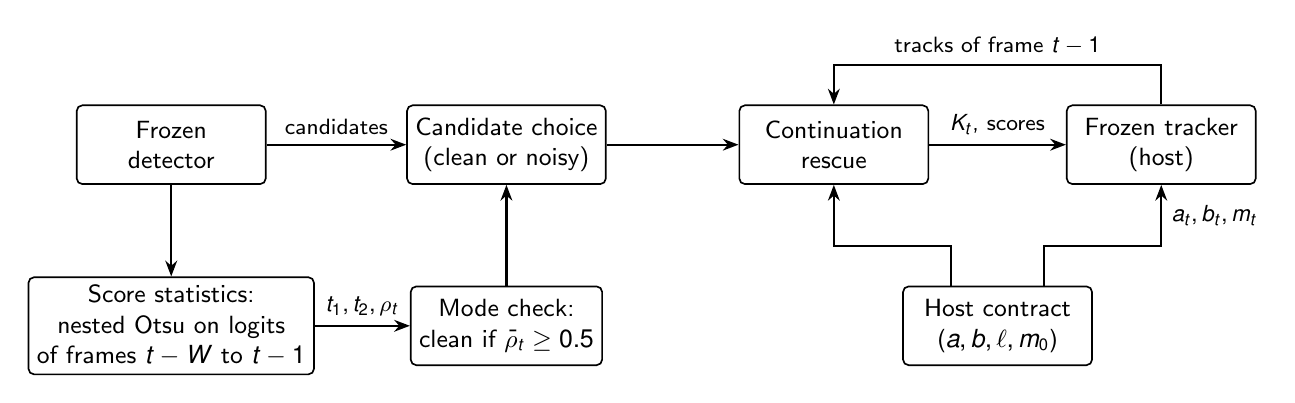
\begin{tikzpicture}[x=0.99cm, y=1cm,
  box/.style={draw, line width=0.6pt, rounded corners=2pt, align=center, font=\small, minimum height=10mm, minimum width=24mm, inner sep=3pt},
  arr/.style={-{Stealth[length=2mm]}, line width=0.8pt}, lab/.style={font=\footnotesize}]
\node[box] (det) at (0,0) {Frozen\\detector};
\node[box] (pol) at (4.3,0) {Candidate choice\\(clean or noisy)};
\node[box] (res) at (8.5,0) {Continuation\\rescue};
\node[box] (trk) at (12.7,0) {Frozen tracker\\(host)};
\node[box] (stat) at (0,-2.3) {Score statistics:\\nested Otsu on logits\\of frames $t-W$ to $t-1$};
\node[box] (reg) at (4.3,-2.3) {Mode check:\\clean if $\bar\rho_t \ge 0.5$};
\node[box] (hc) at (10.6,-2.3) {Host contract\\$(a, b, \ell, m_0)$};
\draw[arr] (det) -- node[lab, above]{candidates} (pol);
\draw[arr] (pol) -- (res);
\draw[arr] (res) -- node[lab, above]{$K_t$, scores} (trk);
\draw[arr] (det) -- (stat);
\draw[arr] (stat) -- node[lab, above]{$t_1, t_2, \rho_t$} (reg);
\draw[arr] (reg) -- (pol);
\draw[arr] (hc.north) ++(-0.6,0) |- ++(0,0.5) -| (res.south);
\draw[arr] (hc.north) ++(0.6,0) |- ++(0,0.5) -| node[lab, pos=0.75, right]{$a_t, b_t, m_t$} (trk.south);
\draw[arr] (trk.north) -- ++(0,0.5) -| node[lab, pos=0.25, above]{tracks of frame $t-1$} (res.north);
\end{tikzpicture}
\end{document}
